\documentclass[11pt,a4paper]{scrartcl}

\usepackage{fullpage}

%\usepackage[ngerman]{babel}
\usepackage[utf8]{inputenc}
\usepackage{graphicx}

\usepackage{amsmath}
\usepackage{amsthm}
%\usepackage{mathtools}

\usepackage{listings}

%%%%% COMMANDS

\newcommand{\FT}{\mathcal{F}}
\newcommand{\T}{\mathrm{T}}
\newcommand{\IFT}{\mathcal{F}^{-1}}
\newcommand{\conv}{\ast}
\newcommand{\defined}{\coloneqq}

\newtheorem*{theorem}{Theorem}

\renewcommand{\thesubsection}{\alph{subsection})}

\begin{document}

\title{Paralleles Höchstleistungsrechnen Übung 1}
\author{Markus Döring, 3153320}
\maketitle

\section{Effiziente Cache-Nutzung}
\subsection{Umordnen von Schleifen}
Die äußere Schleife lässt sich nicht mit einer der inneren Schleifen vertauschen, da 
die Ergebnisse jeder Iteration von denen der vorherigen Abhängen. Damit bleibt nur das 
Vertauschen der inneren Schleifen möglich. In C++ sind die Zeilen eines Feldes zusammenhängend 
im Speicher, daher operiert die Schleife so wie sie ist (von links nach rechts, dann von oben 
nach unten) in Richtung der Cachelines. Die Cacheline links oben wird zum Beispiel nur in den 
ersten 3 Schritten benötigt. Ordnet man die Schleifen jetzt um, dann arbeitet der Algorithmus 
entgegen der Richtung der Cachelines, und nutzt sie somit weniger effizient. Ein Test mit 
einem normalen PC ergab eine Verlangsamung um den Faktor 2.

\subsection{Kachelung}
Das folgende Programm kachelt die Daten und versucht dabei, die Cacheline möglichst effizient 
zu nutzen. Dafür werden zwei 'Kacheln' jeweils ganz in den Cache gelesen. Jede Kachel benötigt 
höchstens die Kachel links und eine Cacheline der Kachel darüber, darum scheint es sinnvoll zwei 
Kacheln gleichzeitig im L1 Cache zu haben. Als Ergebnis mit auf den PC abgestimmten Werten ergab 
sich eine Beschleunigung um Faktor 3.
\newpage
\lstinputlisting[language=C++]{1red.cpp}


\section{ILP}
\subsection{}
Zwischen Zeile 21 und den Zeilen 22/23 besteht eine \emph{Data True Dependence}. Der Hashwert muss erst 
berechnet werden, bevor er als Index benutzt werden kann.

Haben zwei Elemente den gleichen Hashwert, so besteht zwischen den Zeilen 21 der entsprechenden 
Iterationsschritte eine \emph{Data Output Dependence}. Beide Schritte schreiben an eine Speicherstelle, 
die durch den berechneten Hashwert definiert wird (Zeile 33/34). 

Die Variable \emph{ptrUpdate} wird in Zeile 22 berechnet und in Zeile 34 dereferenziert, also gelesen. Damit liegt eine \emph{Data Antidependence} vor. 



% \begin{figure}[ht]
%  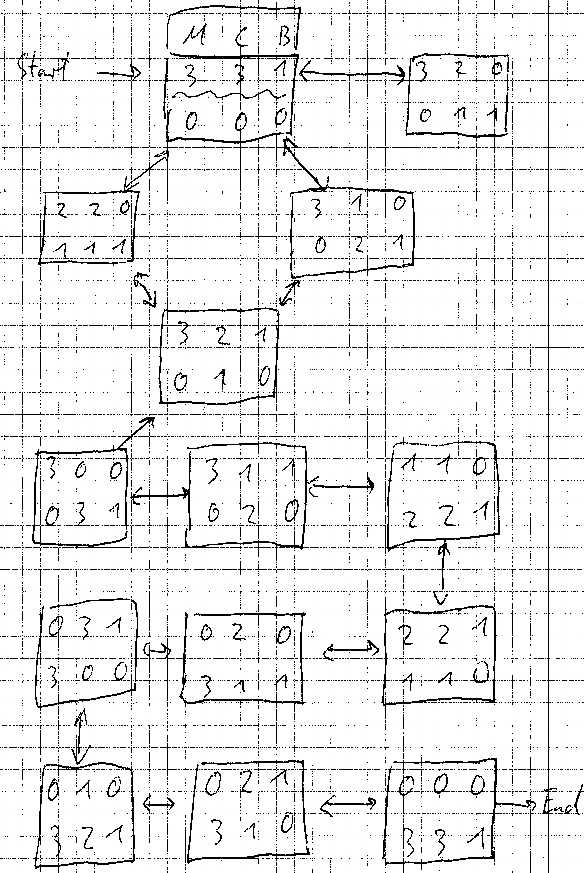
\includegraphics[width=.65\linewidth]{missionaries_cropped.jpg}
%  \caption{The state space graph of the missionary-cannibal-boat problem. The columns denote the objects (M, C, B), the rows the location (side of the river). It turns out that most possible states are not allowed by the problem statement.}
% \end{figure}

%\newpage
%\appendix
%\lstinputlisting[language=python]{ia_05_01.py}
%\newpage
%\lstinputlisting[language=python]{ia_05_02.py}
\end{document}
